\documentclass[compsoc, conference, letterpaper, 10pt, times]{IEEEtran}
\usepackage{graphicx}
\usepackage{amssymb}
\usepackage{amsmath}
\usepackage{amsthm}
% \usepackage{amsart}
\usepackage{bussproofs}
\usepackage{url}
\usepackage{listings}


\newtheorem{definition}{Definition}
%\newtheorem{proposition}{Proposition}
%\newtheorem{thesis}{Thesis}
\newtheorem{theorem}{Theorem}
%\newtheorem{corollary}{Corollary}
%\newtheorem{lemma}{Lemma}


                       \lstset{ %
                       	%backgroundcolor=\color{white},   % choose the background color; you must add \usepackage{color} or \usepackage{xcolor}
                       	%basicstyle=\normalfont\ttfamily,        % the size of the fonts that are used for the code
                       	%basicstyle=\normalfont\footnotesize\ttfamily,        % the size of the fonts that are used for the code
                       	aboveskip={-.4cm},
                       	breakatwhitespace=false,         % sets if automatic breaks should only happen at whitespace
                       	%breaklines=true,                 % sets automatic line breaking
                       	%captionpos=b,                    % sets the caption-position to bottom
                       	commentstyle=\color{Plum},    % comment style
                       	morecomment=[l]{--},
                       	deletekeywords={exp,eq,values,return,room},            % if you want to delete keywords from the given language
                       	escapeinside={(*}{*)},          % if you want to add LaTeX within your code
                       	%extendedchars=true,              % lets you use non-ASCII characters; for 8-bits encodings only, does not work with UTF-8
                       	%frame=single,                    % adds a frame around the code
                       	%keepspaces=true,                 % keeps spaces in text, useful for keeping indentation of code (possibly needs columns=flexible)
                       	%keywordstyle=\color{blue},       % keyword style
                       	language=Java,                 % the language of the code
                       	morekeywords={define,let,cond,if,struct},            % if you want to add more keywords to the set
                      %	numbers=left,                    % where to put the line-numbers; possible values are (none, left, right)
                       	%numbersep=5pt,                   % how far the line-numbers are from the code
                       	numberstyle=\tiny\color{black}, % the style that is used for the line-numbers
                       	%rulecolor=\color{black},         % if not set, the frame-color may be changed on line-breaks within not-black text (e.g. comments (green here))
                       	showspaces=false,                % show spaces everywhere adding particular underscores; it overrides 'showstringspaces'
                       	showstringspaces=false,          % underline spaces within strings only
                       	showtabs=false,                  % show tabs within strings adding particular underscores
                       	%stepnumber=2,                    % the step between two line-numbers. If it's 1, each line will be numbered
                       %	stringstyle=\color{OliveGreen},     % string literal style
                       	tabsize=2,                       % sets default tabsize to 2 spaces
                       	basicstyle=\ttfamily,columns=flexible,
                       	title=\lstname                   % show the filename of files included with \lstinputlisting; also try caption instead of title
                       	%numbers=left,
                       	%basicstyle=\scriptsize,
                       	%mathescape
                       }

\begin{document}
%opening
\title{Simulation of a Trust and Reputation based Mitigation Protocol for a Black Hole Style Attack on VANETs}
%\author{Giuseppe Primiero}
%\institute{Department of Computer Science\\Middlesex University London\\United Kingdom}


\author{

\IEEEauthorblockN{Agostino Martorana}
	\IEEEauthorblockA{Department of Computer Science\\
		Middlesex University London\\
    United Kingdom\\
		Email: am2847@live.mdx.ac.uk}
\and

\IEEEauthorblockN{Giuseppe Primiero}
	\IEEEauthorblockA{Department of Computer Science\\
		Middlesex University London\\
    United Kingdom\\
		Email: G.Primiero@mdx.ac.uk}
\and
\IEEEauthorblockN{Jacopo Tagliabue}
  \IEEEauthorblockA{Tooso Inc.\\
  United States\\
    Email: jacopo.tagliabue@tooso.ai}
    }


\maketitle

\begin{abstract}
From a security standpoint, any VANET (Vehicular ad hoc Network) is a highly flexible network where nodes can freely move and join, with no fixed infrastructure, and thus it is vulnerable to attacks by malicious users. Due to the decentralized and open nature of the wireless system, VANETs are highly prone to various attacks. For many of these kinds of attacks detection is unfeasible, thus making it hard to produce security. Despite their characterization as dynamically reconfigurable networks, it is nonetheless essential to identify topology and population properties that can optimise mitigation protocols' deployment on VANETs. In this paper, we provide a simulation study of a Black Hole stye attack on a VANET and illustrate the use of a previously formally defined trust and mitigation based protocol to contain the attack under well-specified initial conditions.
\end{abstract}


\section{Introduction}\label{sec:intro}

MANET (Mobile Ad hoc Network) refers to a self-configuring system of mobile routers, with wireless links to form an arbitrary topology. The mobility of the routers are provided randomly and organized arbitrarily. VANET (Vehicular Ad hoc Network) is the application of MANET structures to vehicles. and roadside unit networks created to enhance transportation systems through vehicle-to-vehicle (V2V) and vehicle-to-infrastructure (V2I) communications. This kind of systems has various potential applications, such as emergency search and rescue operations, battlefield
communication between moving vehicles and/or soldiers or simply traffic control~\cite{survey1,survey2}.

From a security standpoint, any MANET is a highly flexible network, where nodes can freely move and join, with no fixed infrastructure, and thus it is highly vulnerable to attacks by malicious users. Security of data transmission is the main concern of any MANET. For many of these kinds of attacks, detection is unfeasible, making it hard to produce security. Due to their distributed and dynamic nature, such networks are open to several types of threats, including false message propagation. Trust and reputation are among the  most used concepts to ensure integrity, reliability and safety of services.

While an increasing literature is available on mitigation protocols for such attacks, the focus on dynamic, reconfigurable networks tends to make these results opaque with respect to conditions of the network when the attack takes place. Despite their characterization as dynamically reconfigurable networks, it is nonetheless essential to identify topology and population properties that can optimise mitigation protocols' deployment on VANETs.

The present paper simulates a type of attack on a VANET and deploys a trust and reputation model to mititgate it. Contrary to many contributions in the area, we make use of standard network theory analysis to investigate which network properties (like size and topology), which population properties (like proportion of the attackers) and which contextual conditions (like the current content distribution) are optimal to constraint the attack. This allows to set some clear benchmarks for the specific type of attack we consider; moreover, it makes the model general enough to be easily reconfigured for V2I scenarios. The code of our simulation is made available at \url{https://github.com/gprimiero/trust4vanet2} for reproducibility purposes, together with all data from our experiments.


\section{Related Work}\label{sec:related}


Due to their particular architecture, ad-hoc networks are more easily attacked than wired networks. Two main kind of attacks are usually distinguished~\cite[p.956]{survey3}:

\begin{itemize}
\item  passive attacks: they do not disrupt the operation of the protocol, but try to discover valuable information by listening to traffic;
\item active attacks: they inject arbitrary packets and try to disrupt the operation of the protocol in order to limit availability,
gain authentication, or attract packets destined to other nodes.
\end{itemize}
We focus below on active attacks. The most common type, performed due to their easiness, are ``Attacks Using Modification'': a malicious node disturbs the good operation of an ad-hoc
network by announcing better routes (to reach other nodes or just a specific one) than the other nodes. This kind of attack is based on the modification of the metric value for a route, or executed by
altering control message fields~\cite[p.956]{survey3}. In ``Attacks using Impersonation'' (spoofing), the malicious node hides its real IP address or MAC address and uses another one. As current ad-hoc routing protocols like AODV and DSR do not authenticate source IP address, a malicious node can launch many attacks by using spoofing. For example, a hacker can create loops in the network to isolate a node from the remainder of the network. To do this, the hacker just has to take the IP address of another node in the network and then use it to announce a new route (with the smallest metric) to the others nodes. By doing this, he can easily modify the
network topology as he wants~\cite[p.956]{survey3}. Attacks by ``Resource Overuse'' indicate the additional use of a resource by a node for any activity other than route finding and maintaining or
transmitting data. As mobile nodes may have limited resources in terms of memory, storage, processing power, and battery life, if an IDS involves too much data and computations, then there will be more usage of memory and  processing power, thus disrupting the normal functioning of the network~\cite[p.388]{survey9}.

Several attack strategies can be identified~\cite[p.345]{A}:

\begin{itemize}
\item  \textbf{Black hole Attack}: in this type of attack, malicious nodes broadcast the message to all the nodes,
%, that is has valid, shortest and fresh route to the destination. In this way, such malicious nodes
diverting all the
traffic toward themselves, and without forwarding the data packets to the neighbouring nodes, so that all the (non-malicious) data packets
are dropped;

\item \textbf{Gray hole Attack}: in this form of Black hole attack, the malicious nodes drop the data packets for particular nodes for particular period of time in the network. Gray hole attacks are more difficult to identify as compared to black hole attacks;

\item \textbf{Wormhole Attack}: in this type of attack, two malicious nodes from a tunnel and all the data packets received at one location of the network are tunnelled to the other location, in such a way that all the data are resent to the network. The tunnel between two malicious nodes is called a Wormhole. Such attacks prevent any route other than through the wormhole from being discovered;

\item \textbf{Byzantine Attack}: this type of attack is carried out by intermediate nodes or group of intermediate nodes. Such malicious nodes provide the false routing information and create routing loops as well as forward their data packets to that path which is not optimal and which may be harmful to the system;

\item \textbf{Denial of Service Attack}: it prevents the victim from using all or part of the network connections. DOS attack may have numerous forms and are hard to detect. In this type of attack, attacker nodes send the
excessive amount of data packets or requests to the server so the latter gets busy in testing illegal request and will not be available to other. This attack may degrade the performance of the network since it consumes the
energy (Battery Power) of nodes.
\end{itemize}

Black hole detection has been an active area of research since the `next hop information' based scheme was proposed in 2002~\cite{survey8}, with a
%Researchers have proposed various solutions to identify and handle black hole attacks.
%But merely a
few among the proposed solutions focusing on collaborative black holes. Among the most sophisticated mitigation protocols is the `Fidelity Table' method~\cite{survey6}. In this model, every participating node is allotted a particular fidelity level, a measure of reliability. Whenever a source node broadcasts a RREQ (Route Request) and holds up, the incoming RREPs (Route Reply) are gathered in its Response Table. If the average of the fidelity level of RREP sending node (RREPN) and its next hop node (NHN) in the route is found to be over a predetermined threshold, the RREPN (Route Reply Sending Node) is considered as trustworthy. Therefore, on the receipt of multiple RREPNs, the one with the highest fidelity level is selected. However, if multiple nodes have the same fidelity level, the RREPN with the minimal hop count is
chosen. Finally, routing is accomplished via the selected path. Upon data receipt, the destination node sends an acknowledgement to the source node within timer. Next, fidelity level of the RREPN
is incremented as an accolade for honest routing else that of both RREPN and its NHN is decremented for being collaborative. If fidelity level of a node drops to zero, it is considered as a black hole and the presence of attack is intimated to all using alarm packets. Despite the fact that this method handles both single and collaborative black hole attacks, it involves increased storage overhead, routing overhead, computational overhead and delay. This is because each node should maintain a Fidelity Table and a Response Table that must be updated and exchanged among the
nodes periodically~\cite{survey7}. Reputation is a crucial notion in several other protocols, and used in ours as well.

Reputation is complemented by trust models in several VANET models, defined in accordance to their main object: entity-centric \cite{Minhas:2011:MAM:2334807.2334820, GomezMarmol:2012:TTR:2160992.2161100}, data-centric \cite{DBLP:conf/infocom/RayaPGH08, Lo:2009:RST:1598776.1945486} and combined \cite{Wei2012}. An overview of the issues related to trust in fixed and mobile ad hoc networks is given in \cite{DBLP:conf/vtc/WexBHLD08}, while approaches for trustworthiness and reputation in ad hoc mobile networks are presented, for example, in \cite{DBLP:conf/um/FinnsonZTMC12, DBLP:journals/ijaisc/ChaurasiaTV15}. The work in~\cite{glenford} offers an analysis that accounts for reputation as a characteristic of message forwarding among vehicles, drivers and other agents: reputation of these agents is based on a descriptive ontology and is used to provide feedback in the system. In \cite{DBLP:conf/eurosp/PrimieroRCN17}, we have provided a logic calculus that formally verifies this reputation model by adding a trust function in order to guarantee absence of unsfae behaviours. An interesting way to test the reliability of the model is to simulate an attack, which is the main aim of the present contribution.

\section{The Attack Scenario}\label{sec:attack}

We consider a Black Hole type of attack in which one or more nodes block the transmission of truthful information and start distributing manipulated data. For the present purposes, it is irrelevant the content or dimension of this data and we just represent it by atomic formulas and their negation: an adavanced modelling of the present protocol will focus on the use of real data.

At any point in time in which the attack is deployed, the network can be assumed to have a specific topological configuration produced by the actual set of active communications among its nodes (see Section \ref{sec:network} for the topologies analysed in the present work). A first aim of the present work is to establish which topological structure should the agent have at the moment of the attack (or immediately after) in order to constrain it.

Agents (vehicles) are categorised according to one of three families (or breeds):

\begin{itemize}
\item \textit{discoverers}: one or more agents in possession of truthful and updated data, possibly received by an external network through Internet or a RSU;
\item \textit{attackers}: one or more agents performing the attack, by flipping the truth value of data to be distributed in the network;
\item \textit{receivers}: the remaining set of vehicles, which have no information, or with information requiring an update.
\end{itemize}
Discoverers generate truthful information by assigning truth-value $1$ to a proposition which describe some content of relevance to the network (e.g. ``temperature $<5c$''), according to the routine defined in Figure \ref{fig:discovery}.

\begin{figure}[t]
 	\lstset{language=Java,
	%   numbers=left,
 		basicstyle=\scriptsize,
 		mathescape}
% %
 	\begin{lstlisting}[frame=single]  % Start your code-block

to discovery [ _propositionIndex _#turtles ]
  ask n-of _#turtles turtles [ knowProposition _propositionIndex -1 1 ]
end
\end{lstlisting}
\caption{Discovery}\label{fig:discovery}
%
\end{figure}
Message passing is performed by the routine in Figure \ref{fig:spread}. It requires every agent with a message whose truth value is non-neutral (i.e. equal to either $1$ or $0$) to pass it to one of its neighbors. Note that currently we do not implement the opportuinistic forwarding protocol described in \cite{glenford}, which requires to select the recipient with the highest reputation value.

\begin{figure}[t]
 	\lstset{language=Java,
	%   numbers=left,
 		basicstyle=\scriptsize,
 		mathescape}

    \begin{lstlisting}[frame=single]  % Start your code-block

to spreadKnowledge [ _propositionIndex ]
  ask turtles with [ item _propositionIndex propositions != 0 ]
  [
    let myId who
    let truthVal item _propositionIndex propositions
    ask one-of link-neighbors
    [ knowProposition _propositionIndex myId truthVal ]
  ]
end
\end{lstlisting}
\caption{Message Passing}\label{fig:spread}
%
\end{figure}
By definition, this routine holds for both discoverers and attackers. When an attacker receives truthful information $p$ (labelled by truth-vale $1$) on the current outside temperature and road conditions in view of ice and snow, its aim is to flood the network with its negation (labelled by truth-vale $0$), and to get as many vehicles as possible to distribute it. We implement the attack through the routine defined in Figure \ref{fig:attack}.

\begin{figure}[t]
 	\lstset{language=Java,
	%   numbers=left,
 		basicstyle=\scriptsize,
 		mathescape}
% %
 	\begin{lstlisting}[frame=single]  % Start your code-block

  to attack [ _propositionIndex ]
    ask n-of number_attacker turtles with
       [ item _propositionIndex propositions = 1 ]
    [
      set breed attackers
      knowProposition _propositionIndex -2 -1
    ]
  end
\end{lstlisting}
\caption{Attack}\label{fig:attack}
%
\end{figure}
If no protocol is in place to resolve conflicting information transmission, the attack might easily succeed. This is clearly shown by the initial experimental results in Section \ref{sec:experiments}. If a simple majority protocol is used to discern between conflicting data, it might be enough for the attacker to target a limited number of nodes with high degree of connectivity, in order to flood the entire network. Trust and reputation are crucial to improve on simple quorum protocols.

Several of the work presented in Section \ref{sec:related}, introducing trust and reputation methods for VANET attacks, presents such attacks under the general assumption that the network is dynamic and therefore no topological analysis is usually done. As a negative effect, this means that results are usually under-specified with respect to which are the initial conditions (topological, temporal, etc.) of the attack. Our main aim is to investigate whether the trust and reputation protocol presented in \cite{DBLP:conf/eurosp/PrimieroRCN17} is effective in preventing such type of attacks under precise and well specified conditions, including which should be the preferred topological structure of the network in the aftermath of an attack in order to limit its efficacy. In particular, our parameters concern:
\begin{enumerate}
\item the topology of the network at the moment of the attack;
\item the proportion of discoverers and attackers;
\item the ranking of truthful information object of the attack;
\item the state of truthful information diffusion at the moment of the attack.
\end{enumerate}

\section{The Trust and Reputation Model}\label{sec:model}

$\mathtt{(un)SecureND}$ is a natural deduction calculus introduced in \cite{DBLP:conf/pst/PrimieroR14} to define trust, mistrust and distrust protocols and extended in \cite{DBLP:conf/ifiptm/Primiero16} with a negation connective. In \cite{DBLP:conf/eurosp/PrimieroRCN17} a modified version has been presented, adapted for a VANET network with the introduction of a reputation measure.

Given $\mathcal{A}$ a set of agents containing vehicles $\mathcal{V}$ and roadside units (RSUs) $\mathcal{R}$, an order $\prec$ holds between agents and expresses a reputation order. $\mathcal{S}$ denotes a set of services for the messages, with $\mathcal{C}$ a set of service characteristics, and each element $C^{S_i}_{\overrightarrow{n}}$ denoting the set of $n$ characteristics of service $S_{i}$. In general, characteristics $C^{S_i}_{\overrightarrow{n}}$ of services for each service $S_i$ are associated with an order $\leq$ used to order messages, and for two characteristics
$C^{S_{i}}_{\overrightarrow{n}}, C^{S_{j}}_{\overrightarrow{n}}, i\neq j$, there is no order between them. In the present experimental analysis, we limit ourselves to a single message $p$ about a given service with one characteristic. The analysis of the model generalised to multiple messages concerning several characteristics for one service is left to future research.

In the implementation, we translate an order relation $p_{i}<p_{j}$ between messages as a fixed absolute ranking value of a unique message $p$ (\texttt{rank p}), which we will assume is shared by all vehicles in each messaging instance, and can assume three distinct numerical values corresponding to low, medium and high relevance. As a further simplification, we assume atomic messages, although the underlying logic $\mathtt{(un)SecureND}$ allows for closure under connectives. For any given message $p$ received from another agent (either vehicle or RSU), a vehicle will collect all the formulas that follow from accepting it. This is called the Feedback Set of an agent with respect to a message. In view of the mentioned simplification, our Feedback Set is always a singleton. The vehicle assigns a value to this atomic formula, using three parameters:
\begin{enumerate}
\item a fixed ranking of the source, generated in this model automatically by the topology of the network (see below Section \ref{sec:network} for more details);
\item a ranking of the message, fixed at some low, medium or high value for each messaging operation;
\item the time at which the reception of the message occurs, computed by the clock underlying the simulation (the later the message arrives, the more updated it is considered, the highest its value).
\end{enumerate}
We call the resulting value \texttt{Apperception}, see Figure \ref{fig:routine1}. As a result of working with atomic messages only, the Apperception of a vehicle for a message is computed by unary factors. Using this value, we define directly the order of reputation for agents, which establishes a higher position for the vehicle whose apperception is greater.

\begin{figure}[t]
 	\lstset{language=Java,
	%   numbers=left,
 		basicstyle=\scriptsize,
 		mathescape}
% %
 	\begin{lstlisting}[frame=single]  % Start your code-block

to-report calculateApperceptionValue
[ sourceRanking _propositionRanking _tick ]
  report (1.0*sourceRanking)*(1.0*_propositionRanking)*(_tick*1.0)
end
\end{lstlisting}
\caption{Apperception}\label{fig:routine1}
%
\end{figure}
%
% \begin{definition}[Reputation]
% $\forall v_{i}, v_{j}\in \mathcal{V}, S_{i}\in \mathcal{S}, v_{i}\prec v_{j} \leftrightarrow AP^{v_{i}}(\mathcal{M}^{\mathcal{A}}_{S_{i}, C_{k}})>AP^{v_{j}}(\mathcal{M}^{\mathcal{A}}_{S_{i}, C_{k}})$.
% \end{definition}

\subsection{Network Construction}\label{sec:network}

As mentioned, the original model which inspires the present implementation and presented in \cite{glenford} uses reputation to define a recipient selection protocol: after $v_{i}$ broadcasts a `hello' message, if both $v_{k}, v_{j}$ receive and accept the message, then $v_{i}$ has to select a reciepient on the basis of the reputation order between $v_{k}$ and $v_{j}$. Accordingly, a new profile is built out of $v_{i}$ and the higher of the two recipients, thus modelling a communication channel.

In the present implementation, given fixed network topologies we assign an agent ranking on their basis. Reputation then is defined by this factor together with message ranking and timing, as explained above. In particular, we consider the three following main topologies and associated agent ranking methods:

\begin{itemize}
\item \textit{small-world}: the network is generated according to a power-law, by which each new node has a higher probability to be linked to a node with high in-degree than to one with low in-degree; in this topology, higher in-degree nodes have higher ranking;
\item \textit{total}: every node is connected to any other node, and all have the same ranking;
\item \textit{random}: edges are randomly distributed, and so is the ranking which reflects the in-degree of each node.
\end{itemize}
The advantage of fixing the networks and of determining the agent ranking on that basis is to experimentally evaluate the optimal topological conditions for the mitigation protocol. A next step of this protocol evaluation will implement reputation (based on message ranking and timing only) as a criterion for recipient selection.

\subsection{Message Passing Protocol}

The trust protocol from the logic $\mathtt{(un)SecureND}$ enforces a consistency check on message passing. Each valid vehicle profile meets all the requirements and conflicts clauses of all service messages that the vehicle receives. Trust allows to select valid messages among those that are read: if a message is received by a vehicle and it preserves its profile consistency, then it can be trusted. A message readable and trustable by a vehicle can be further broadcast to other vehicles. Mistrust is the protocol acting on conflicting messages: a currently held message conflicting with a newly arrived message is removed from the current vehicle profile and none of its consequences are included; any message consistent with the conflict resolution is trusted by removal of the mistrusted message in the vehicle profile, including any required dependency.

In the present implementation, message passing with consistent information or when the receiving agent is an attacker is unproblematic: it induces respectively acceptance and rejection of the new message (in the latter case, it means an attacker once flipped the value of a received message will no longer change it). Message passing consistent information to an agent who has no prior information induces a reputation control: information is accepted when coming from a source with higher reputation, while the receiver remains undecided if information comes from a source with lower reputation. A conflict is generated by two contradictory messages, and the profile is valid when such conflicts are avoided. Receiving contradictory information requires again reputation checking: with a source that has reputation at least as high as the receiver, the latter checks with any linked agent with higher reputation than the source; when these show consensus (see Figure \ref{fig:consensus}) with the receiver about its currently held information, the latter does not change its mind, and it does otherwise. See Figure \ref{fig:passing1}.


\begin{figure}[t]
 	\lstset{language=Java,
	%   numbers=left,
 		basicstyle=\scriptsize,
 		mathescape}
% %
 	\begin{lstlisting}[frame=single]  % Start your code-block

to-report verifyProposition
[ _currentVal _newVal _propositionIndex _breed _currentWho _sourceWho]
  if (_breed = attackers)
     [ report _currentVal ]
  if (_currentVal = _newVal)
     [ report _newVal ]
  if (_currentVal = 0)
  [  ifelse (sourceApperception >= currentApperception)[ report _newVal ]
    [ report 0 ]
  ]
  if (_currentVal $!=$ _newVal)
  [  ifelse (sourceApperception $>=$ currentApperception)
    [ let consensus
      neighborConsensus _propositionIndex _newVal sourceApperception
      ifelse (consensus = false) [ report _currentVal ]
      [ report _newVal ]
    ]
    [ report _currentVal ]
  ]
  \end{lstlisting}
  \caption{Trust}\label{fig:passing1}
  %
\end{figure}


\begin{figure}[t]
 	\lstset{language=Java,
	%   numbers=left,
 		basicstyle=\scriptsize,
 		mathescape}
% %
 	\begin{lstlisting}[frame=single]  % Start your code-block

  to-report neighborConsensus
  [ _propositionIndex _truthVal _sourceApperception ]

    let total_neighbors_with_opinion count link-neighbors with
    [item _propositionIndex propositions != 0
    and item _propositionIndex apperception > _sourceApperception]

    let total_neighbors_with_same_opinion count link-neighbors with
    [item _propositionIndex propositions = _truthVal
    and item _propositionIndex apperception > _sourceApperception ]

    if (total_neighbors_with_opinion = 0) [ report false]
    report total_neighbors_with_opinion = total_neighbors_with_same_opinion
  end
  \end{lstlisting}
  \caption{Consensus}\label{fig:consensus}
  %
\end{figure}
%
%


\section{Experimental Results}\label{sec:experiments}

To experimentally validate our mitigation protocol, we have considered the following parameters:

\begin{enumerate}
\item \textit{network topology}: we investigate the optimal topology among small-world, total and random newtorks for the minimization of the attack's effects;
\item \textit{network size}: we consider three main values on this parameter, with networks of $10,50,100$ nodes;
\item \textit{message ranking}: a static value at each message passing operation, valid for all agents (both discoverers and attackers), investigated with three different values $0.20, 0.50, 0.80$ corresponding respectively to \texttt{low,medium,high} ranking;
\item \textit{proportion of discoverers}: proportion of agents with truthful information at the beginning of the protocol, investigated with three values $10\%, 50\%, 90\%$;
%, which in combination with the proportion of attackers and the network size provide us with a sufficiently differentiated number of configurations;
\item \textit{proportion of attackers}: proportion of agents performing an attack, investigated with two values $1\%, 10\%$ (experimentally shown to be the lower and higher bound required for optimization);
\item \textit{network coverage for attack}: coverage of the entire newtork with truthful information when the attack is executed, investigated with three values $20\%, 50\%, 80\%$ corresponding respectively to \texttt{low,medium,high} coverage (reflecting an early, intermediate and late attack).
\end{enumerate}

All experiments reported below have been executed on a machine with 7.7 GB of memory, 64bit Ubuntu 17.10 system, NetLogo 6.0. Each configuration has been run for a minimum of 100 times, and for several configurations we have run 10 repetions of 100 runs each. The results report the median values of all runs.

\subsection{First Configuration: Topology and Size}

In the first set of experiments, we focus on determining optimal topology and size for our mitigation protocol. We investigate all sizes and topologies while keeping message ranking and network coverage parameters both at a minimum level (respectively $0.20$ and $20\%$).

Our first experiment is executed with a proportion of attackers and of discoverers both fixed at $10\%$, i.e.\ with respectively $1,5,10$ attackers/discoverers on networks of $10,50,100$ nodes. Results are plotted in Figure \ref{fig:plot1}: it clearly illustrates how the attack is highly successful and the protocol has only limited efficacy.

\begin{figure}
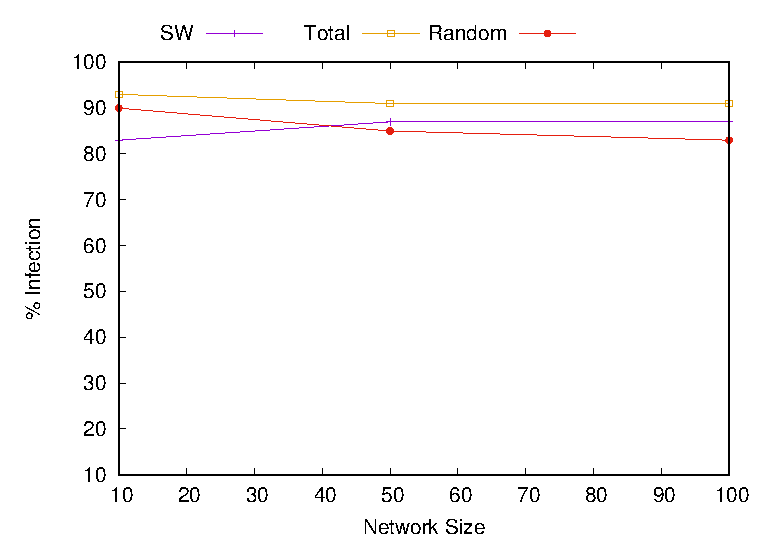
\includegraphics[scale=0.70]{1stconfig}
\caption{Experiment 1: Attack with $10\%$ attackers/discoverers.}\label{fig:plot1}
\end{figure}
These values tend to decrease sensibly when varying the proportion between attackers and discoverers, in a way which preserves in general the optimality of the topologies. By fixing the proportion of attackers at $1\%$ (in general, this means we are reducing the attacker to $1$), but increasing the proportion of discoverers to $90\%$, we find that the protocol makes the network a lot more resilient to the attack, see Figure \ref{fig:plot2}.

\begin{figure}
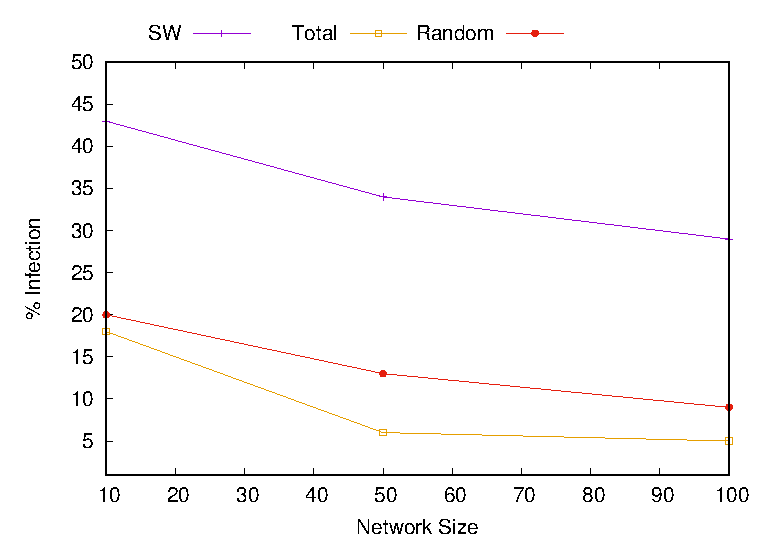
\includegraphics[scale=0.70]{1stconfig_1_90}
\caption{Experiment 2: Attack with $1\%$ attackers and $90\%$ discoverers.}\label{fig:plot2}
\end{figure}
Performed -- but not reported here -- experiments cover several in-between configurations confirming these maximal and minimal configurations. These initial findings show that, while there is a positive effect intrinsically generated by the network size (the greater the network, the harder to spread the attack), it is sufficient for the attackers breed to cover $10\%$ of the entire population in order to nullify such advantage. On the ohter hand, with a single attacker, size sensibly helps reducing the infection, with a totally connected network presenting the most advantageous setting for the mitigation protocol, followed by random and small-world. This suggests that in a dynamically reconfigurable network, if an attack is identified or suspected, total connectivity should be sought by the agents (vehicles and RSU) in order to minimize its negative effects.

\subsection{Second Configuration: Message Ranking}

The second set of experiments focuses on how the ranking of the message affects the ability of the protocol to constraint the attack. We show how rising the value of \texttt{rankp} from $0.2$ to $0.5$ in the setting of the first experiment (Figure \ref{fig:plot1}) has an immediate positive effect, bringing a drastic improvement in small newtorks of $10$ nodes, and a significant one also in larger configurations, see Figure \ref{fig:plot3}. Further rising the value of \texttt{rankp} to $0.8$ does not improve these results.

\begin{figure}
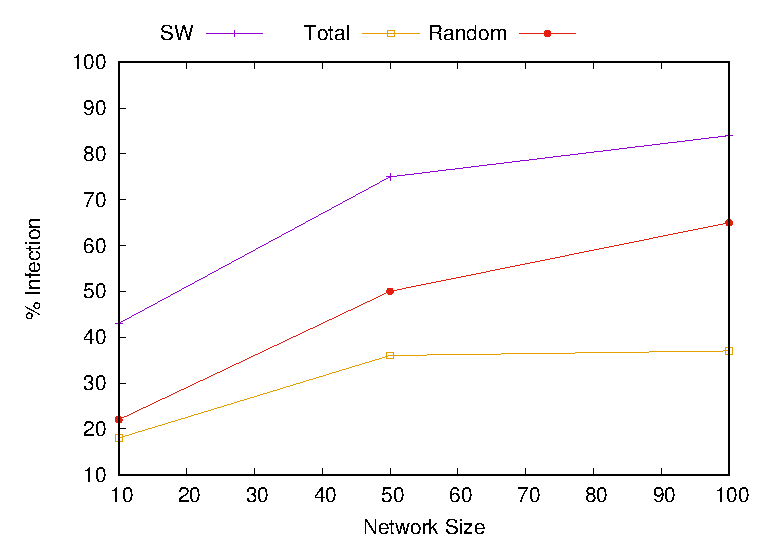
\includegraphics[scale=0.70]{3rdconfig_10_90}
\caption{Experiment 3: Attack with $10\%$ attackers/discoverers and $0.5$ message ranking.}\label{fig:plot3}
\end{figure}
On the other hand, preserving the best results from the first configuration, thus analysing small-world, total and random networks with a single attacker and a proportion of $90\%$ discoverers (i.e. the configuration of Experiment 2 in Figure \ref{fig:plot2}), while rising the level of the variable \texttt{rankp} from $0.2$ to $0.5$ and $0.8$, it is possible to show that rising message ranking has no influence in further reducing the infection in all topologies. These results suggest that reputation is only partially influenced by the relevance of the message, as this obviously is computed for both discoverers and attackers. Future experiments should focus on the difference to this factor provided by messages concerning different characteristics within the same service.


\subsection{Third Configuration: Network Coverage}

The third set of experiments focuses on how the infection is effected when parametrised by the relation between the attack being struck and a percentage of the network having already received  truthful data. We show in Figure \ref{fig:plot4} the results for the setting of the first experiment (Figure \ref{fig:plot1}) modified by rising the value of  \texttt{network\_coverage} from $0.2$ to $0.8$. There is again a drastic improvement in small newtorks of $10$ nodes, and a significant one in larger configurations.

\begin{figure}
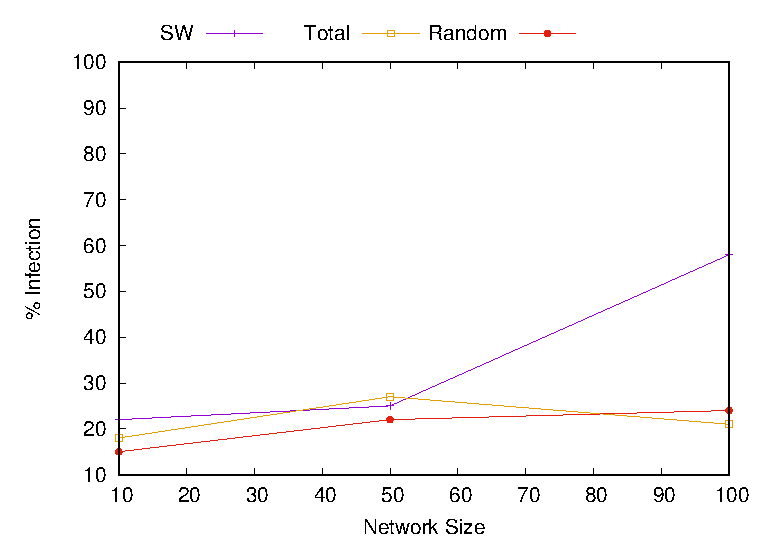
\includegraphics[scale=0.70]{4thconfig_10_90}
\caption{Experiment 4: Attack with $10\%$ attackers/discoverers and $0.8$ network coverage.}\label{fig:plot4}
\end{figure}
Note that, again, preserving the best results from the first configuration, thus analysing small-world, total and random networks with a single attacker and a proportion of $90\%$ discoverers (i.e. the configuration of Experiment 2 in Figure \ref{fig:plot2}), while rising the level of the variable \texttt{network\_coverage} from $0.2$ to $0.8$, no significant improvement in the results is obtained. These results suggest that damage limitation after an attack of the present type requires an elevated number of nodes connected to an external network, to facilitate the increase of agents with updated information at any point.

\subsection{Fourth Configuration: Combined Optimal Parameters}

In the last set of experiments, we combine the optimal message ranking and network coverage parameters. We first observe this combination in the non-optimal setting of experiment 1 (Figure \ref{fig:plot1}), i.e.\ with a proportion of attackers and of discoverers both fixed at $10\%$ on networks of $10,50,100$ nodes. The results are plotted in Figure \ref{fig:plot5}, which shows how this configuration manages to keep the infection below $25\%$ in the largest networks and presents an average decrease in infection of over $75\%$ across the three topologies, when compared with the worst-case scenarion of experiment 1.

\begin{figure}
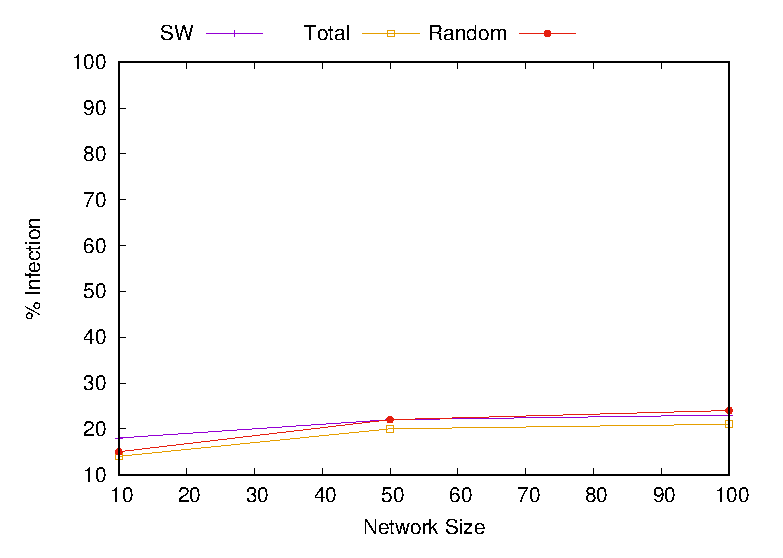
\includegraphics[scale=0.70]{5thconfig}
\caption{Experiment 5: Attack with $10\%$ attackers/discoverers, $0.5$ message ranking and $0.8$ network coverage.}\label{fig:plot5}
\end{figure}
Finally we consider how the optimal configuration of message ranking and network coverages affects the results of Experiment 2 (Figure \ref{fig:plot2}), where the proportion of attackers is minimised to $1\%$ and that of discovered maximised to $90\%$. Results shown in Figure \ref{fig:plot6} illustrate how the protocol is able to minimise the negative impact of an attack by a single agent on networks with a large proportion of agents who transmit the truthful data if messaging ranking and network coverage are optimised. The average improvement on the result on the same networks without these last two parameters optimised is of almost $30\%$ across all topologies.

\begin{figure}
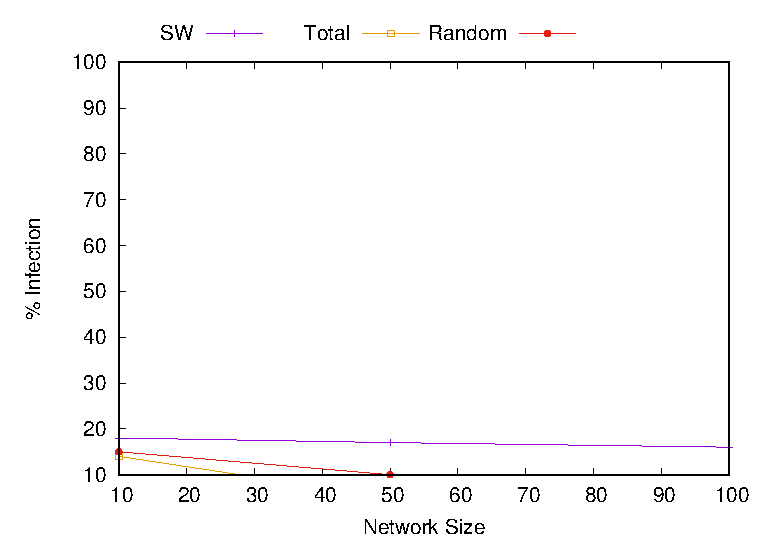
\includegraphics[scale=0.70]{5thconfig_1_90}
\caption{Experiment 6: Attack with $1\%$ attackers, $90\%$ discoverers, $0.5$ message ranking and $0.8$ network coverage.}\label{fig:plot6}
\end{figure}

\subsection{Summary of Results}

The results from the experiments can be summarised as follows:
\begin{itemize}
\item the reputation protocol is essential in constraining the attack on networks of any size with at least $10\%$ of the population acting as attackers (an improvement of up to $80\%$ on the same conditions without reputation);
\item the protocol is up to $90\%$ more efficient in a one-attacker condition;
\item total networks are overall the most efficient topology for attack mitigation and, in general, network size is relevant only when considered in absence of the reputation protocol.
\end{itemize}

\section{Conclusions}

%In this paper we have formulated a proof-theory
In this paper we have provided a simulated analysis of a trust and reputation based protocol for the mitigation of Black Hole type attacks in VANETs. The present implementation is simplified under several aspects, in particular: messaging is a one-time event and is not repeated in short time spans; message forwarding happens by random recipient selection; messages are atomic. Nothwistanding this specification, our analysis clearly shows under which initial topological and population conditions is the protocol efficient.

Our next steps for this research include: the implementation of a lower level of abstraction in the protocol, including repeated broadcasting and opportunistic forwarding; the translation to a simulation environment that can help capture such relevant properties, like OmNet++ or VSimRTI; testing the protocol on real data, which will be made available thanks to the testbed deployed by colleagues at Middlesex University~\cite{10.1007/978-3-319-49580-4_8}.

\medskip

%\noindent {\em Acknowledgement.}

%
\bibliographystyle{plain}
\bibliography{vanetattack.bib}


\end{document}
